%!TEX root = ../dokumentation.tex

\chapter{Stand der Technik}
In diesem Kapitel werden bisherige Forschungsarbeiten mit ähnlichen Ansätzen vorgestellt und mit dieser Arbeit in den Kontext gestellt. Es wurden bereits mehrere alternative Steuermöglichkeiten zu den herkömmlichen VR-Controllern erforscht und erprobt. 

\section{Interaction techniques using head gaze for virtual reality}
\label{paper1}
Diese im Mai 2016 veröffentlichte Arbeit hat sich zum Ziel gesetzt, die Position des Kopfes zu nutzen, um die ungefähre Blickrichtung des Nutzers zu erkennen und somit natürlichere Interaktionen in der virtuellen Realität zu ermöglichen. Die Motivation hinter der Arbeit war es, die doch sehr unnatürliche Steuerung über Controller zu ersetzen, um so eine bessere Immersion in die virtuelle Welt zu gewährleisten. Die Wahl, die Kopfbewegung als Steuerung zu nutzen, ist gefallen, da diese Bewegung von allen natürlcih vorkommenden interaktiven Bewegungen eines Nutzers (wie z.B. Handbewegungen, Augenbewegungen, Fuß/Beinbewegungen und Kopfbewegungen) am einfachsten zu erfassen und in VR übertragbar ist. Da ein Großteil der VR-Headsets auf dem Erfassen des Kopfes in einem Raum basiert (TODO vgl Kpaitel von Jörn wie er des erklärt), ist die Erfassung dieser Daten meist ohne größere Umstände möglich. Um ein Aussagekräftiges Ergebnis zu erlangen, wurden mehrere Versuchsreihen und anschließende Befragungen der Probanden durchgeführt. Die Autoren der Arbeit haben dafür einige Spiele (teils bereits in VR existierend, teils Portierungen von Smartphone Spielen in VR) so angepasst, dass Kopfbewegungen zur Steuerung eingelesen werden können. Als Eingabegeräte wurden ein Leap Motion Controller (ein Hand-Tracking Gerät), ein herkömmlicher XBox Controller und das von den Autoren "Head Gaze" benannte Kopf-Tracking miteinander verglichen. Als VR-Headset wurde ein Oculus DK2 verwendet. 
Nach der ersten Versuchsreihe in dem Spiel "Slash the Fruit VR" hat sich Head Gaze als die intuitivste Eingabemethode herausgestellt. Daher wurden in den nachfolgenden beiden Versuchen mit den Spielen "Virtual Reality Experience" (kurz VREx) und "Dungeon VR" nur noch Head Gaze verwendet. Der Grund hierfür war zum Einen die Unzuverlässigkeit des Leap Motion Controllers, zum Anderen war der XBox Controller nicht intuitiv genug für Bewegungen in VR. 
Da die Kernfrage die Immersion der neuen Steuerung war, wurden die Teilnehmer der Versuchsreihe nach ihrem Immersionsbefindnis befragt.

\begin{figure}
	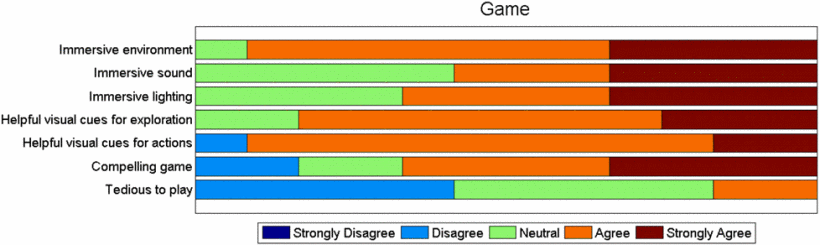
\includegraphics[width=\linewidth]{images/study1immersion}
	\caption{Resultat der Befragung}
	\label{fig:result1}
\end{figure}

Wie in den oben stehenden Ergebnissen zu sehen ist, empfand der Großteil der Nutzer diese Steuerung als immersiv und nur wenige Nutzer haben sich von der Steuerung gestört gefühlt. Als weiteres Ziel der Forscher wird von den Forschern eine Umsetzung in Smartphone VR-Anwendungen erwähnt.
\subsection{Einordnung der Relevanz}
Die beschriebene Arbeit ist für den in dieser Arbeit vorgesehenen Versuchsaufbau von großer Relevanz, da es zu einem gewissen Grad eine Vorstufe darstellt. Der Begriff Head Gaze wird von den Forschern bewusst verwendet, da mit der Kopfbewegung auch der Blick (engl. Gaze) angenommen werden kann. Somit sind der Versuchsaufbau und die damit einhergehenden Ergebnisse sehr gut mit den in dieser Arbeit entstandenen Ergebnissen vergleichbar. (TODO Vergleich) 
\section{Electrooculogram-based virtual reality game control using blink detection and gaze calibration}
Diese im September 2016 vorgestellte Arbeit beschreibt die Verwendung von einem Elektrookulogramm zur Bestimmung der Blickrichtung und zum Erkennen von Blinzeln. Diese Daten werden dann als Eingabe in einem VR-Spiel verwendet. 
Ein Elektrookulogramm (EOG) ist die Registrierung von Bewegungen der Muskeln, die zur Kontrolle der Augen dienen. Dabei werden an jeder Seite der Augenhöhle außerhalb Elektroden angebracht, mit welchen die Bewegung der Augen und Augenlider aufgezeichnet werden kann. 
Wie schon in Kapitel~\ref{paper1}, lag auch hier das Ziel dabei, eine intuitivere und immersivere Eingabemethode zu entwickeln. Zur Überprüfung der Ergebnisse werden sowohl die Rate der falschen Eingaben als auch die subjektive Empfindung erfasst. Als Beispielapplikation wird das Spiel "VRrailSurfer" verwendet. Das Spielprinzip ist vergleichbar mit dem bekannten Smartphone Spiel "Subway Surfers" Eine Bewegung der Augen nach links oder rechts hat eine Bewegung der Spielfigur in die entsprechende Richtung zur Folge. Zum Springen müssen die Augen nach oben bewegt werden. Die mit dieser Methode erzielte Genauigkeit der Steuerung lag nach einer Reihe von Versuchen mit 10 Probanden im Durchschnitt bei 78\%, wohingegen die Blinzelerkennung mit 96\% deutlich höher lag. Die Forscher haben allerdings in diesem Beispiel nur die Steuerung über den Blick im Spiel implementiert, sie gehen aber davon aus, dass eine Genauigkeit von rund 96\% auch in einem Spiel mit Blinzelerkennung umsetzbar ist. 
\subsection{Einordnung der Relevanz}
Das Paper ist für diese Arbeit auch relevant. Trotz der komplett anderen Eye-Tracking Methode sind einige Punkte auf diese Arbeit übertragbar. Der Ansatz, Augenbewegungen über ein EOG zu erfassen, ist allerdings eher suboptimal, da die Genauigkeit nicht so hoch ist, wie bei dem in dieser Arbeit verwendeten System, da mehr Komplikationen, wie etwa ein verrutschen der Elektroden, auftreten können. Der Fokus des Papers lag allerdings eher auf der Machbarkeit eines EOGs in Verbindung mit einem VR-Headset, weshalb kein Vergleich mit anderen Eingabemethoden stattgefunden hat. 

\section{Eye-Gaze-Controlled Telepresence Robots for People with Motor Disabilities}

\subsection{Einordnung der Relevanz}

\section{Behavior Analysis of Indoor Escape Route-Finding Based on Head-Mounted VR and Eye Tracking}

\subsection{Einordnung der Relevanz}

\section{VR-HMD Eye Tracker in Active Visual Field Testing}

\subsection{Einordnung der Relevanz}

\section{Eye-gaze-triggered Visual Cues to Restore Attention in Educational VR}

\subsection{Einordnung der Relevanz}

